\chapter{Conclusion}
\label{ch:conclusion}

% TODO short recap introduction
% TODO hypothesis
% TODO what introduced
% TODO result of hypothesis
In the introduction, we presented shape completion as the problem of reconstructing
an individual object given a partial observation, \eg from a single view.
We argued that shape priors play a crucial role in shape perception
in general \cite{Pizlo:2007,Pizlo:2010} and shape completion in specific.
We also outlined the recent success in learning shape models using deep generative models,
\eg in \cite{GirdharGupta:2016,BrockWeston:2016,WuSongXiao:2015,WuTenenbaum:2016},
and the use of shape priors for data-driven shape completion
\cite{DameReid:2013,EngelmannStuecklerLeibe:2016,EngelmannLeibe:2017}.
Learning-based approaches to shape completion, in contrast, directly
learn shape completion in a supervised setting
\cite{SmithMeger:2017,DaiNiessner:2016,SharmaFritz:2016,
FanSuGuibas:2016,RezendeHeess:2016,RieglerGeiger:2017}, most of them using deep neural networks.
While these approaches allow efficient inference, \ie shape completion is
``just a forward pass'' in the trained network, their applicability is limited
by the requirement of annotated training data. Data-driven approaches
are directly applicable to real data by posing shape completion -- and thereby
inference -- as energy minimization. We hypothesized that using generative
shape models enables us to learn shape completion in an unsupervised setting.
As result, shape completion would still be efficiently performed by a trained
network while avoiding the need of annotated datasets.

With the goal to learn shape completion of cars on KITTI
\cite{GeigerLenzUrtasun:2012,GeigerLenzStillerUrtasun:2013}, we proposed
and implemented two probabilistic frameworks in order to experimentally
test our hypothesis. In particular, based on a variational auto-encoder
as shape prior, we posed shape completion as maximum likelihood problem
over the learned latent space -- in the spirit of \eg \cite{EngelmannStuecklerLeibe:2016}.
Following the idea of amortized inference, we 
then trained an encoder to directly predict maximum likelihood solutions,
\ie learning an embedding of observations within the latent shape space,
by interpreting the maximum likelihood objective as unsupervised loss.
As alternative approach, we also considered directly integrating the observations
as random variable within the latent variable model, \ie within the
variational auto-encoder. Considering the corresponding joint distribution
allowed us to derive an evidence lower bound and train an extended variational
auto-encoder implicitly also learning shape completion. Both approaches
can be trained on KITTI using cars from ShapeNet
\cite{ChangFunkhouserGuibasSavarese:2015} for the shape prior. Furthermore,
shape completion, \ie inference, is efficiently done by the trained network.
Experimentally, we showed that both approaches optimize a similar objective.
On a synthetically generated, ShapeNet-based dataset we showed that both
are able to compete with a fully-supervised baseline, both quantitatively and
qualitatively. On KITTI, we demonstrated that the proposed approaches are,
indeed, applicable to real data and can learn shape completion in an 
unsupervised setting.

%\begin{figure}
%  \centering
%  \hspace*{-1cm}
%  \begin{tikzpicture}
%    \node at (0, 0) {
%      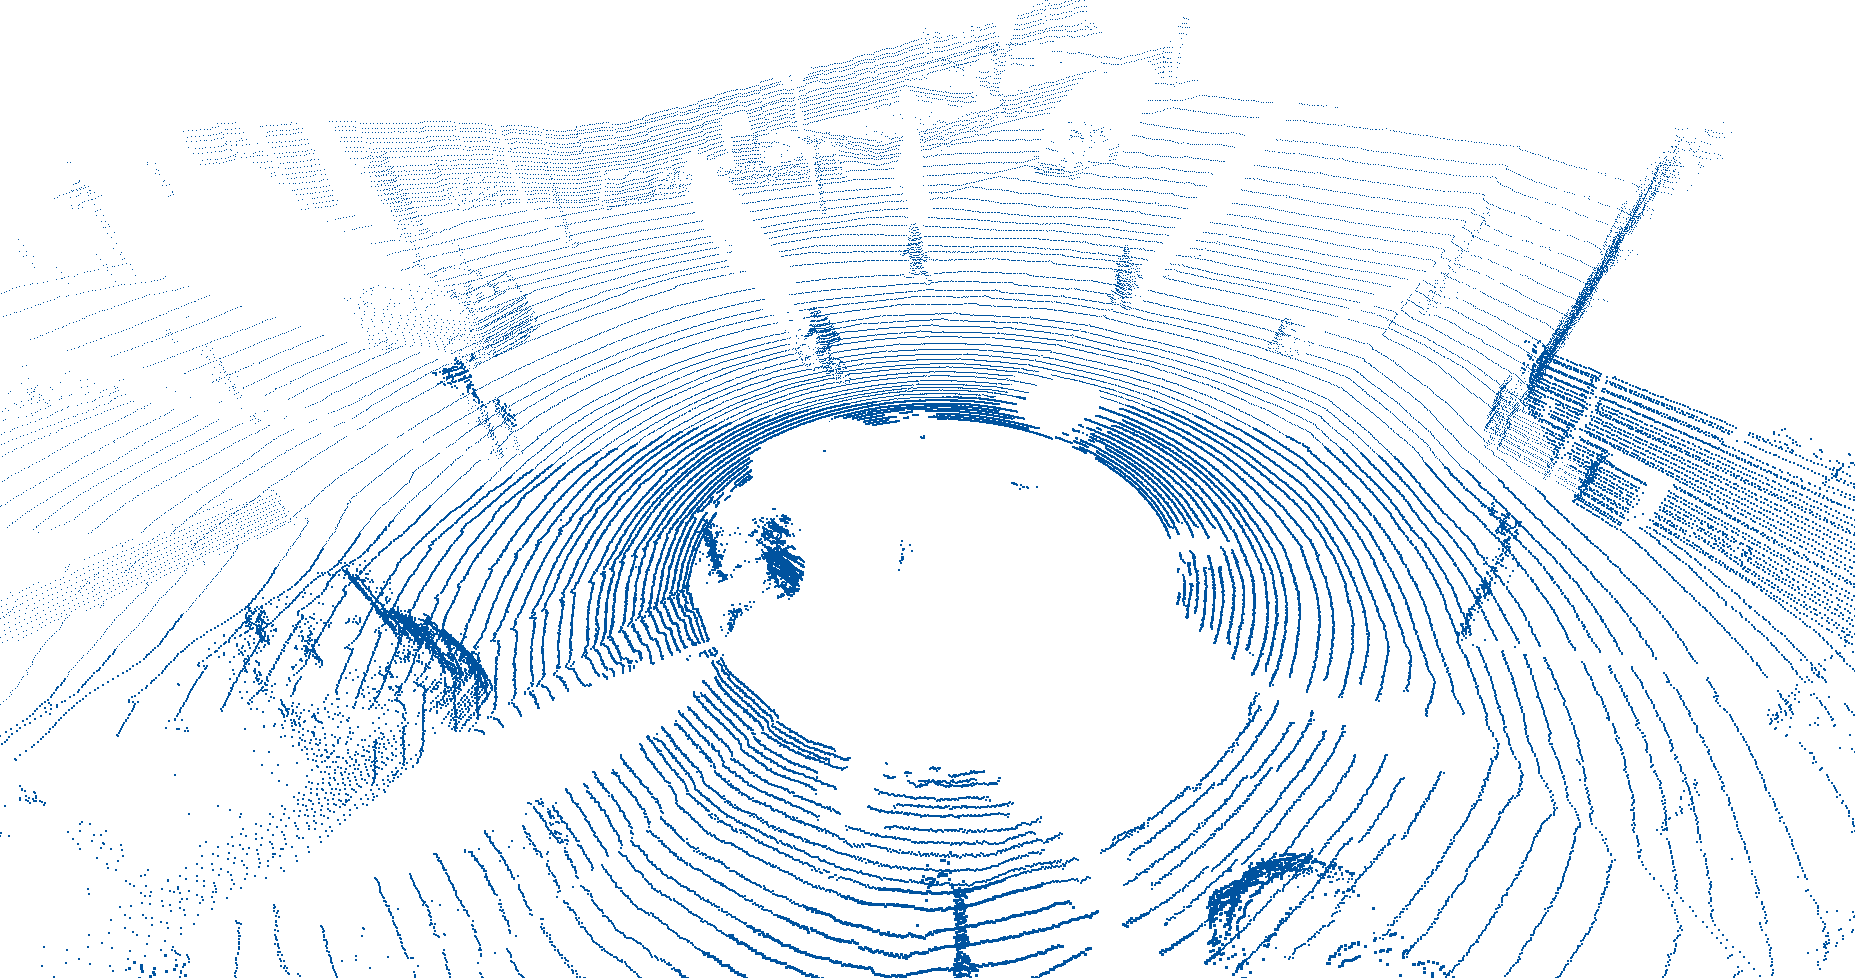
\includegraphics[width=7.5cm,trim={0 0 6cm 6cm},clip]{experiments/kitti/vae_occ_aml/15_long_statistics_combined/snapshot00}
%    };
%    \node at (8, 0) {
%      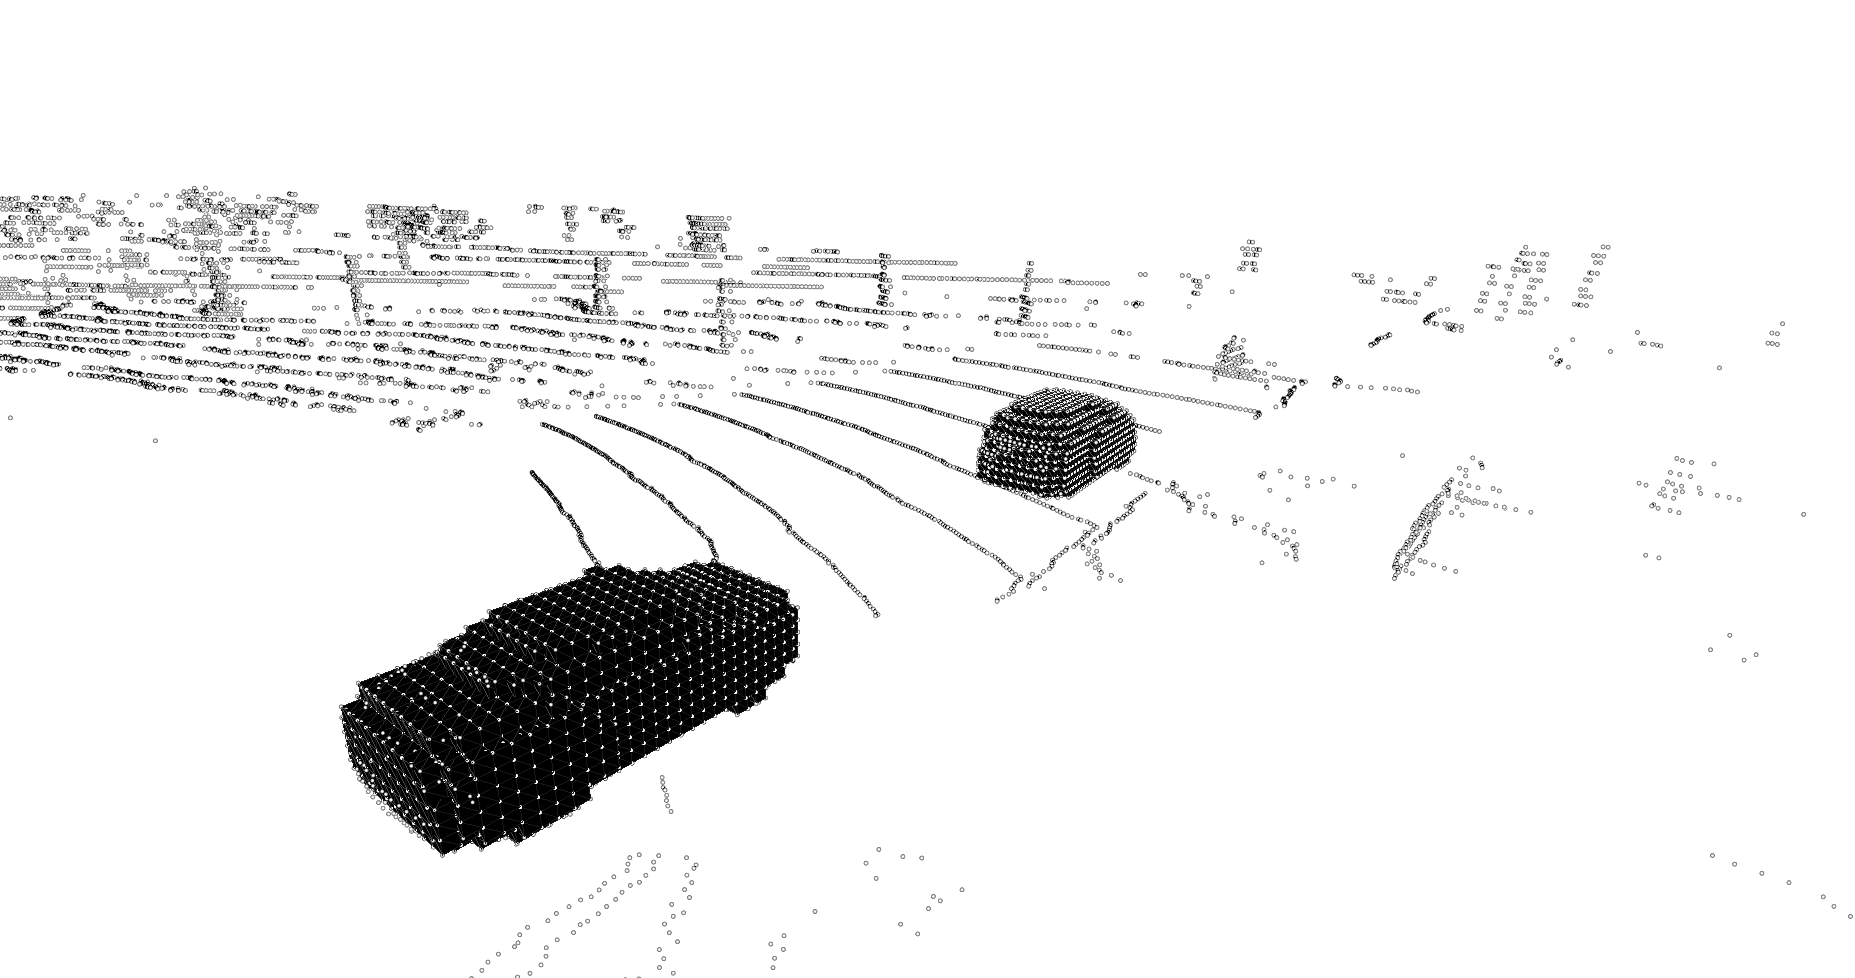
\includegraphics[width=7.5cm,trim={0 0 6cm 6cm},clip]{experiments/kitti/vae_occ_aml/15_long_statistics_combined/snapshot02}
%    };
%  \end{tikzpicture}

  % TODO short caption
%  \caption{An illustration of our experimental results on KITTI
%  \cite{GeigerLenzUrtasun:2012,GeigerLenzStillerUrtasun:2013}. Here,
%  we used the proposed amortized maximum likelihood framework to
%  complete cars using the provided ground truth 3D bounding boxes.
%  The corresponding shape prior was trained on ShapeNet
%  \cite{ChangFunkhouserGuibasSavarese:2015}. We
%  subsequently back-projected the completed shapes into the original,
%  raw point clouds to show that the estimated shapes fit the overall
%  scale and orientation.}
%  \label{fig:conclusion}
%\end{figure}

In conclusion, the presented experiments are in favor of our hypothesis
that strong shape priors allow to learn shape completion without supervision.
We believe this to be an important first step in reasoning about shapes as well
as scenes in a weakly-supervised manner by explicitly using strong shape priors
that can be learned on synthetic data. Finally, the presented results also
pose new questions going beyond the scope of this work -- some of which
we will discuss in the following.

\section{Future Work}
\label{sec:future-work}

% TODO non-cubic resolution
% TODO experiments w.r.t. uncertainty
% TODO advantage of learning inference vc baseline? Learning color too? learning instance segmentation too?

% TODO subvoxel accuracy: predicting real signed distance functions
% TODO Bernoulli PPCA
% TODO model p(x|y) using knowledge about rendering process in EVAE
% TODO evae with y -> x rendering module
% TODO inverting evae
% TODO experiments not done: longer training time, parameter tuning, monitoring
We believe that the
presented work poses many interesting new research questions.
Within the proposed frameworks we are \eg interested in replacing the
used ground truth 3D bounding boxes with 3D detections from a state-of-the-art
object detector or extending the presented experiments to consider
true signed distance functions allowing to derive more accurate and detailed meshes.
Considering the extended variational auto-encoder, we can imagine directly
learning the observation model from synthetic data or explicitly modeling
real sensors, \eg KITTI's Velodyne sensor.
It might also be worthwhile to investigate the limitations of the proposed approaches
in more details. For example, how many observations we need to
learn proper shape completion and whether the prior is able to express ambiguity
in terms of uncertainty within the predictions. In comparison to the baseline it
is also interesting to consider additional advantages of learning shape completion
on real data, \eg by additionally learning color (given enough observations)
or a figure-ground segmentation of the provided observations.
To further improve the ability to predict more detailed shapes,
we might also consider related work for learning in higher resolutions,
\eg octree-based approaches \cite{RieglerGeiger:2016,RieglerGeiger:2017,TatarchenkoBrox:2017}
or PointNet-based architectures \cite{QiSuGuibas:2016a,FanSuGuibas:2016,QiYiSuGuibas:2017}.
As we are currently also limited to one object category, we would like
to extend the proposed frameworks to consider multiple object categories
at ones, \eg on other real datasets such as SUNRGBD \cite{SongXiao:2015}
and thereby also experiment with different modalities (\ie RGB-D images from
Kinect-like sensors compared to KITTI's Velodyne sensor).

